%%=============================================================================
%% Inleiding
%%=============================================================================

\chapter{\IfLanguageName{dutch}{Functionele Omschrijving TAC2.0}{Functional Description TAC2.0}}
\label{ch:functionele-omschrijving}

Het checkoutsysteem van Colruyt Group, \textbf{FVS} (``filiaalverkoopsysteem''), bestaat uit een verscheidenheid aan individuele componenten en is verwoven met zo goed als elk domein binnen de firma — gaande van marketing en customer management tot herbevoorrading en accountancy. Een grondige kennis van dit systeem, en in het bijzonder de werking van de kassa vanuit het perspectief van de kassabediende, is dan ook onontbeerlijk voor dit onderzoek.

\section{TAC Hardware}

Kassabedienden en verkopers in de filialen van Colruyt, Colruyt France, OKay, OKay City, Bio-Planet, Dreamland, Dreambaby, en Colruyt Group Spar zijn kennen het checkoutsysteem vooral als ``de \textbf{TAC}''. ``TAC'' komt van het Engelse woord ``tactile'' en verwijst naar het feit dat het scherm voornamelijk bediend wordt door er op te tikken met de vingers.

\subsection{Opstellingen}

Er zijn grosso modo 2 verschillende opstellingen:

\begin{enumerate}
     \item \textbf{Gescheiden}. Het registreren en afhandelen van klantenaankopen gebeurt in twee stappen. In de eerste stap worden zijn aankopen geregistreerd, alsook worden eventuele kortingsbonnen en klantenkaarten aan de rekening toegevoegd. Het TAC-scherm dat daarvoor gebruikt wordt, staat bekend als de \textbf{CTAC} ('C' voor ``controle''). De betaling vindt vervolgens plaats aan een tweede scherm, gekend als de \textbf{PTAC} ('P' voor ``payment''). De klanten van Colruyt, OKay en Bio-Planet zijn vertrouwd met deze opstelling.
     \item \textbf{Gecombineerd}. Het is ook mogelijk om het volledige kassaproces aan één TAC-scherm af te ronden, zoals in OKay City, Dreamland, Dreambaby en Colruyt Group Spar winkels gebeurt. In dat geval wisselt het systeem tussen het registratiescherm en het betaalscherm, afhankelijk van de gebruikssituatie. Er zijn meerdere opstellingen die aan dit profiel voldoen, met name de \textbf{MTAC} ('M' voor ``multi'') en de \textbf{KTAC} ('K' voor ``\emph{k}ombinatie''). Hun onderlinge verschillen worden niet verder behandeld.
\end{enumerate}

\begin{figure}%
    \centering
    \subfloat{{\includegraphics[width=6cm]{img/func-omsch/CTAC-OKay-Overzetten.jpg} }}%
    \qquad
    \subfloat{{\includegraphics[width=6cm]{img/func-omsch/PTAC-OKay.jpg} }}%
    \caption{Links: CTAC opstelling, rechts: PTAC opstelling — beide in het OKay opleidingslokaal op de Wilgenveld site in Halle.}%
    \label{fig:ctac-ptac-okay}%
\end{figure}

\subsection{Randapparaten}

Een TAC opstelling is voorzien van enkele randapparaten (``peripherals''), afhankelijk van het soort TAC opstelling dat gebruikt wordt:

\begin{itemize}
    \item \textbf{3D barcodelezer} — wordt gebruikt voor het inlezen van artikelbarcodes, pakketten, kortingsbonnen en klantenkaarten. De barcodelezer wordt niet voorzien aan een PTAC opstelling.
    \item \textbf{Tafelscanner} — alternatief voor de barcodelezer dat in het kassameubel van Dreamland, Dreambaby en sommige Spar winkelformules ingebouwd wordt.
    \item \textbf{Kaartlezer} — ingebouwd in de TAC hardware. Laat toe klantenkaarten in te lezen aan de hand van hun magneetstrook. Dit apparaat wordt zelden gebruikt, maar laat wel toe om klantenkaarten met een betaalfunctie in te lezen aan de PTAC.
    \item \textbf{Weegschaal} — wordt niet voorzien aan een PTAC opstelling of in de \emph{non-food} winkelformules (Dreamland en Dreambaby).
    \item \textbf{Klantendisplay} — geeft de klant informatie over de geregistreerde items aan de PTAC in Colruyt, OKay en Bio-Planet. In Spar winkels geeft het klantendisplay ook informatie over het betalingsverloop.
    \item \textbf{Lamp} — een Colruyt CTAC opstelling gebruikt een hangende lamp boven de winkelkar als visuele feedback op artikelregistraties.
    \item \textbf{Betaalterminal} — laat betalingen met debet-, krediet-, en maaltijdcheque kaarten toe. Klanten die met een interne betaalkaart (Xtrakaart met betaalfunctie, Colruytkaart) betalen, gebruiken de terminal ook om hun geheime code in te tikken.
    \item \textbf{Geldlade} — PTAC en MTAC/KTAC configuraties sturen ook de geldlade aan, die ze kunnen openen en wiens sluiting ze ook kunnen detecteren.
\end{itemize}

\subsection{Gebruikersinterface}

%%%TODO

\section{Systeemarchitectuur}

De high level systeemarchitectuur van FVS wordt geschetst in figuur \ref{fig:FVSHighLevel}.

\begin{figure}[h!]
    \centering
    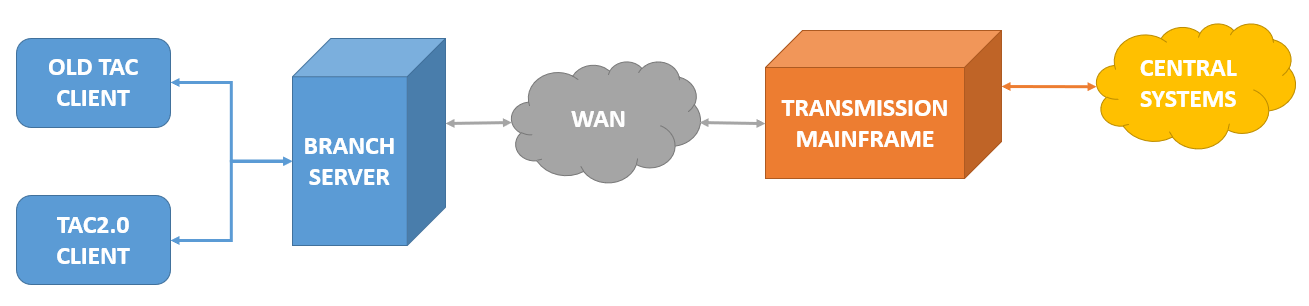
\includegraphics[scale=0.35]{img/func-omsch/DiagramHighLevel.PNG}
    \caption{High level view van FVS, het checkoutsysteem van Colruyt Group.}
    \label{fig:FVSHighLevel}
\end{figure}

Elk filiaal beschikt over één \textbf{filiaalserver} die met de centrale systemen communiceert. Afhankelijk van de richting van die communicatie spreekt men binnen Colruyt Group over ``mutaties'', ``transmissies'' of over ``online transacties''.

\begin{itemize}
    \item Een \textbf{mutatie} is het versturen van data van een centraal systeem naar één specifieke filiaalserver, waaronder artikeldata (het assortiment en prijzen), promoties, en de gegevens van klantenkaarten. Dit kunnen kreaties [sic], wijzigingen, of eliminaties zijn.
    \item Een \textbf{transmissie} is de omgekeerde beweging en gaat voornamelijk over verkoopsgegevens (kastickets, voorraadwijzigingen etc.). Mutaties en transmissies gebeuren voornamelijk 's nachts, hoewel sommige soorten (dringende correcties) ook tijdens de operationele uren gebeuren.
    \item \textbf{Online transacties} zijn ten slotte (meestal synchrone) web services voor tijdgevoelige communicatie, zoals het controleren van klantenkaarten en het afhandelen van betalingen met de Xtra of Colruyt kaart.
\end{itemize}

De FVS filiaalserver communiceert nooit rechtstreeks met de centrale systemen; de \textbf{transmissie mainframe} neemt de verantwoordelijkheid voor het valideren en formatteren van mutaties, het initiëren en afhandelen van transmisies, en biedt aan FVS een service (\emph{ProcessBranchRequest}) aan voor online transacties.

Figuur \ref{fig:FVSDetail} modelleert de filiaalserver en zijn onmiddellijke context.

\begin{figure}[h!]
    \centering
    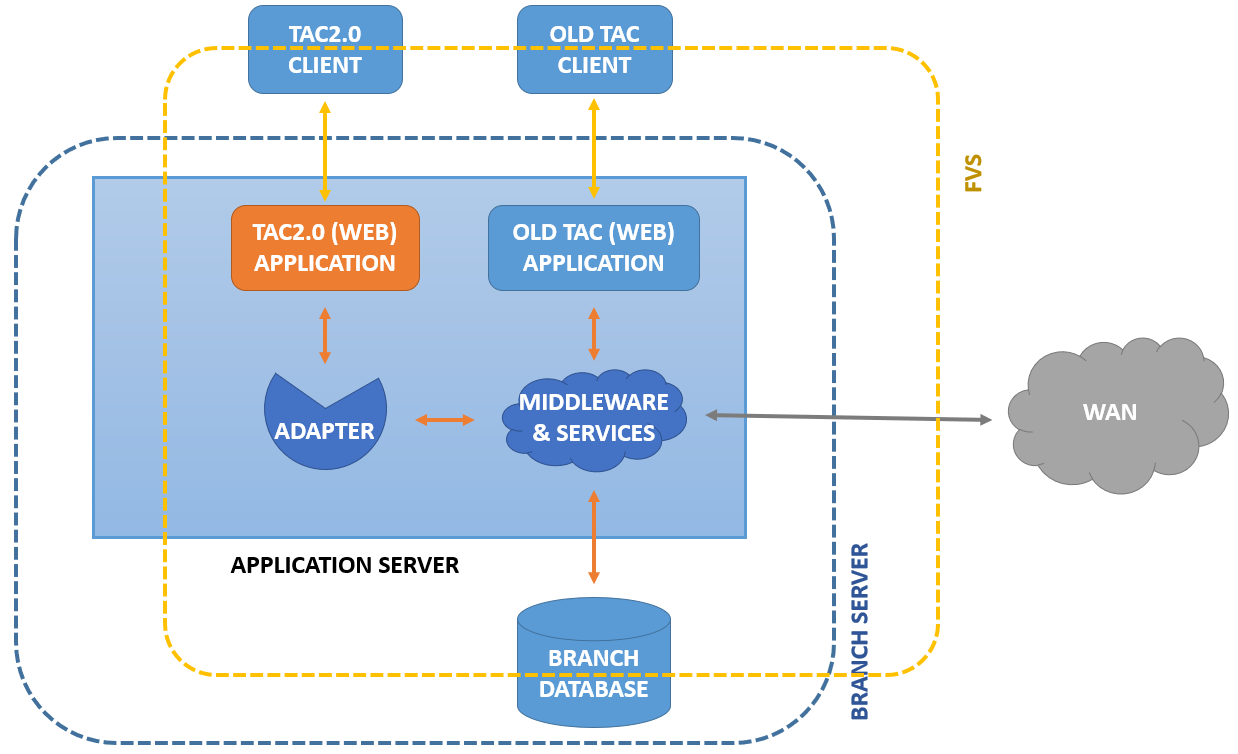
\includegraphics[scale=0.35]{img/func-omsch/DiagramLowerLevel.PNG}
    \caption{Gedetailleerd overzicht van de architectuur van de filiaalservers die Colruyt Group gebruikt.}
    \label{fig:FVSDetail}
\end{figure}

De frontend van het kassasysteem, zowel de huidige versie als de toekomstige TAC2.0 versie, is een webapplicatie die op de (lokale) filiaalserver draait. De TAC client is een ``lege doos'' die bij opstart zijn basisconfiguratie ontvangt van de cradle waar deze op aangesloten zit, en vervolgens een image van zijn stripped-down besturingssysteem download van de filiaalserver. Dit laat toe om TAC schermen te wisselen zonder manuele configuratiewijzigingen.

De TAC client navigeert, middels een browser (Chromium in het geval van TAC2.0), naar het adres van deze webapplicatie bij de opstart van de client. Deze webapplicatie wordt gehost op een Websphere application server die runt op de filiaalserver. Naast de webapplicatie zelf, runnen een reeks middleware applicaties en services eveneens op de virtuele applicatie server.

Deze middleware en services worden aangeroepen door de TAC frontend om diverse taken te voltooien, waaronder het registreren van transacties, het afhandelen van een elektronische betaling, en het activeren van geschenkkaarten. De TAC2.0 webapplicatie gebruikt op het moment van schrijven een adapter om deze middleware en services te kunnen gebruiken, hoewel die laatsten op termijn ook herschreven zullen worden.

Tot slot runt de filiaalserver ook een databank, die voornamelijk gebruikt wordt door het FVS systeem. Zoals figuur \ref{fig:FVSDetail} suggereert, zijn er nog andere toepassingen die gebruik maken van de applicatie server en de databank die zich op de filiaalserver bevinden. Dit zijn voornamelijk winkelapplicaties die hier niet verder besproken worden.

\section{Functionaliteiten}

Colruyt Group is een sterk procesgerichte organisatie; 

Registreren en afhandelen van klantenaankoop < Verkopen van goederen < Verkoop

speciale barcodes